\documentclass[12pt,a4paper]{article}
\usepackage[T1]{fontenc}
\usepackage[utf8]{inputenc}
\usepackage[spanish]{babel}
\usepackage{amsmath}
\usepackage{amsfonts}
\usepackage{amssymb}
\usepackage{graphicx}
\usepackage{cite}
\usepackage[hidelinks]{hyperref}
\usepackage{geometry}
\usepackage{caption}
\captionsetup{font=footnotesize}
\geometry{a4paper, margin=2.5cm}

\title{Avance Preliminar: Proyecto Teórico}
\author{Mateo Rubio Hernández}
\date{\today}

\begin{document}

\maketitle

%\begin{abstract}
%Este documento presenta una revisión preliminar de los conceptos transversales del Mezclado de Cuatro Ondas (FWM) en medios atómicos, con un énfasis particular en el modelado teórico de la competencia entre este proceso no lineal y la Emisión Espontánea Amplificada (ASE). Se estudian las configuraciones de los niveles de energía, las ecuaciones de matriz de densidad y el fenómeno de interferencia cuántica destructiva que rige la supresión de la población en niveles excitados.
%\end{abstract}

\section{Introducción al Mezclado de Cuatro Ondas (FWM)}
El Mezclado de Cuatro Ondas (FWM, por sus siglas en inglés) es un proceso óptico no lineal de tercer orden en el cual tres campos electromagnéticos interactúan dentro de un medio no lineal para generar un cuarto campo. Este fenómeno está regido por la susceptibilidad no lineal de tercer orden del medio $\chi^{(3)}$ y requiere el cumplimiento simultáneo de la conservación de la energía y del momento (condición de ajuste de fase o \textit{phase-matching}) \cite{Becerra2008}.

Físicamente, la interacción de los campos incidentes induce una polarización macroscópica no lineal en el medio que oscila y actúa como fuente para la nueva onda electromagnética. Para modelar esta interacción luz-materia a nivel atómico, se emplean las ecuaciones ópticas de Bloch y el formalismo de la matriz de densidad, el cual permite estudiar la evolución temporal de las coherencias y las poblaciones atómicas considerando efectos como la desintonía, la relajación transversal y el decaimiento espontáneo \cite{Documento2025}.

\section{El Caso Especial: Competencia entre ASE y FWM}
Uno de los fenómenos más notables de la dinámica no lineal es la competencia 
entre procesos ópticos. En el trabajo de Boyd et al. (1987) se estudia la excitación 
por medio de la absorción de dos fotones del nivel 3d en un átomo de sodio y 
observaron una fuerte competencia entre la ASE y el proceso de FWM paramétrico \cite{Boyd1987}.

A simple vista, los cálculos teóricos de ganancia independiente sugieren que la ASE 
debería ser el proceso dominante de forma abrumadora en el medio. Sin embargo, las observaciones 
experimentales muestran que el proceso de FWM es capaz de suprimir por completo la aparición de
la ASE.

Para comprender por qué surge esta supresión, es necesario recurrir a la solución perturbativa de las ecuaciones de la matriz de densidad, cuyas expresiones analíticas se detallan en el Anexo \ref{density_matrix}. El formalismo de la matriz de densidad permite aislar el comportamiento de las coherencias inducidas por los campos ópticos y calcular la transferencia fraccional hacia los distintos niveles de energía. El análisis de estos elementos revela que los campos electromagnéticos generados por el propio proceso de FWM crean un camino de excitación cuántica secundario que conecta el estado fundamental con el nivel excitado de dos fotones.

La conclusión central del trabajo de Boyd y sus colaboradores establece que estos múltiples caminos de excitación sufren una interferencia destructiva. A medida que los campos paramétricos del FWM se propagan y crecen en el medio de acuerdo con las condiciones de acoplamiento de fase, el término de interferencia cruzada entre el láser de bombeo aplicado y los campos generados cancela la amplitud de probabilidad neta de la transición atómica.

\begin{figure}[ht]
    \centering
    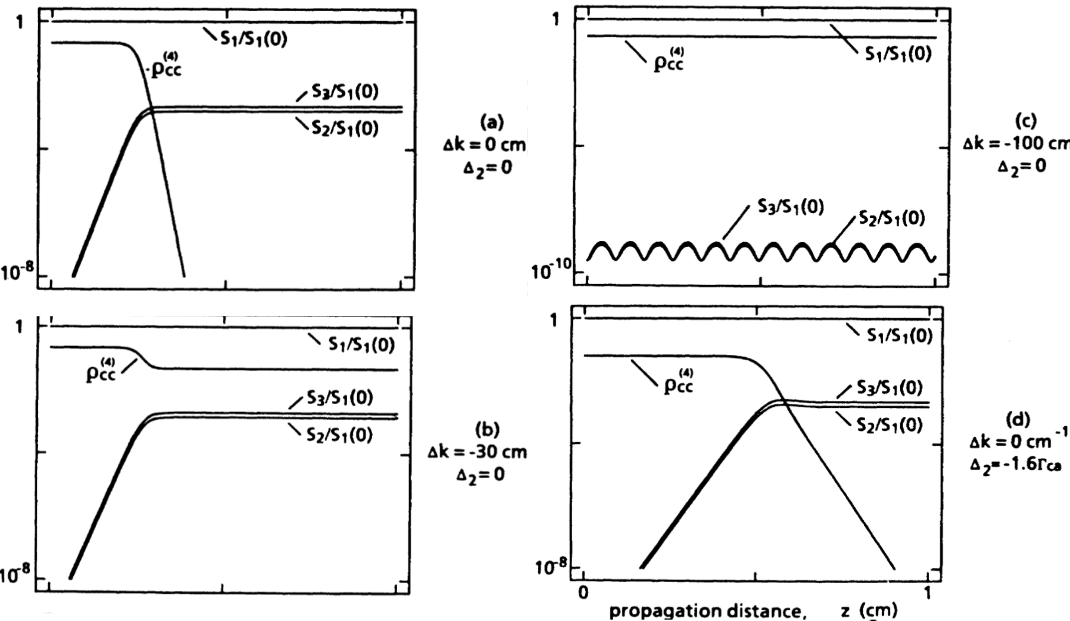
\includegraphics[width=0.85\linewidth]{rhocc.png}
    \caption{Evolución espacial de la población del nivel excitado $\rho_{cc}^{(4)}$ y de las intensidades normalizadas de los campos ópticos en función de la distancia de propagación $z$. Los cuatro paneles ilustran la dinámica del sistema ante diferentes condiciones del desacople de fase $\Delta k$ y la desintonía de dos fotones $\Delta_2$. En el panel (a), bajo condiciones de acoplamiento de fase perfecto ($\Delta k = 0$) y resonancia exacta ($\Delta_2 = 0$), se observa cómo la población $\rho_{cc}^{(4)}$ se anula a medida que los campos se propagan a través del medio. Los paneles (b) y (c) demuestran que, al introducir un error en el acoplamiento de fase, la interferencia pierde efectividad. El panel (d) muestra que el acoplamiento de fase perfecto es capaz de anular la población incluso fuera de resonancia exacta. Imagen modificada de \cite{Boyd1987}.}
    \label{rhocc}
\end{figure}

Esta interferencia destructiva conduce a un estado estacionario donde la población del nivel superior excitado $\rho_{cc}$, desciende exactamente a cero, tal como se puede observar en la Figura \ref{rhocc}. La relación entre esta falta de población y el dominio del FWM radica en los requisitos fundamentales de cada fenómeno. La Emisión Espontánea Amplificada es un proceso que requiere intrínsecamente que exista una gran cantidad de átomos físicamente excitados en el nivel superior para iniciar el decaimiento radiativo y la posterior amplificación en cascada. 

Al anularse la transferencia de población hacia dicho nivel debido a la interferencia, el medio atómico queda sin la fuente material de fotones espontáneos, bloqueando de raíz el mecanismo de la ASE. Por el contrario, el FWM es un proceso impulsado por las coherencias atómicas, no por la permanencia física de los electrones en el estado superior. Al suprimirse la absorción real de energía hacia el nivel excitado, el sistema canaliza la energía incidente a través de la polarización macroscópica, favoreciendo exclusivamente la generación de los campos del FWM.

\bibliographystyle{unsrt}
\bibliography{referencias_fwm}

\newpage
\appendix
\section{Anexo: Soluciones Perturbativas de la Matriz de Densidad}
\label{density_matrix}

En este anexo se presentan las expresiones analíticas detalladas por Boyd et al. (1987) para los elementos de la matriz de densidad, calculadas mediante la teoría de perturbaciones. Estas ecuaciones describen la evolución de un sistema atómico de tres niveles bajo la aproximación de onda rotatoria (RWA) y asumiendo un estado estacionario.

\subsection*{Orden Cero: Condición Inicial}
Antes de la interacción con los campos ópticos, se asume que toda la población atómica reside en el estado fundamental $a$, y que no existen coherencias previas en el sistema:

\begin{equation}
\rho_{aa}^{(0)} = 1 \tag{1a}
\end{equation}
\begin{equation}
\rho_{lm}^{(0)} = 0 \quad (\text{para } l \neq m \text{ y para } l = m \neq a) \tag{1b}
\end{equation}

\subsection*{Primer Orden: Absorción Lineal}
El primer orden de perturbación representa la interacción de un solo fotón. Crea una coherencia entre el estado fundamental $a$ y el nivel intermedio $b$, lo que da origen a la polarización lineal del medio:

\begin{equation}
\rho_{ba}^{(1)} = \frac{\mu_{ba}}{\hbar} \left[ \frac{\tilde{E}_1 e^{-i\omega_1 t}}{\Delta_1 - i\Gamma_{ba}} + \frac{\tilde{E}_2 e^{-i\omega_2 t}}{2\Delta_1 - \Delta_3 - i\Gamma_{ba}} + \frac{\tilde{E}_3 e^{-i\omega_3 t}}{\Delta_3 - i\Gamma_{ba}} \right] \tag{2}
\end{equation}

\begin{itemize}
    \item $\mu_{ba}$ es el elemento de matriz del momento dipolar eléctrico de la transición $a \leftrightarrow b$. Junto con la amplitud del campo eléctrico incidente, define la frecuencia de Rabi de la interacción, parametrizando la fuerza del acoplamiento luz-materia.
    
    \item $\Delta_1$ y $\Delta_3$ son las desintonías ópticas de los campos $\omega_1$ y $\omega_3$ respectivamente. Se definen como la diferencia entre la frecuencia de transición atómica pura y la frecuencia del láser incidente (ej. $\Delta_1 = \omega_{ba} - \omega_1$). 
    
    \item $2\Delta_1 - \Delta_3$ es la desintonía efectiva que experimenta el campo generado $\omega_2$. Esta combinación lineal de desintonías surge de la conservación de energía del proceso que impone que la frecuencia del nuevo campo debe ser $\omega_2 = 2\omega_1 - \omega_3$.
    
    \item $\Gamma_{ba}$ representa la tasa de relajación transversal a la cual se destruye la coherencia cuántica entre los niveles $a$ y $b$.
\end{itemize}

\subsection*{Segundo Orden: Coherencia de Dos Fotones}

Al incorporar una segunda interacción electromagnética, se establece una coherencia entre el estado fundamental $a$ y el estado superior $c$.
 
\begin{equation}
\begin{aligned}
\rho_{ca}^{(2)} &= \frac{\mu_{cb}\mu_{ba}}{\hbar^2} \left[ \frac{\tilde{E}_1^2 e^{-i2\omega_1 t}}{(\Delta_1 - i\Gamma_{ba})(\Delta_2 - i\Gamma_{ca})} \right. \\
&\quad + \frac{\tilde{E}_2\tilde{E}_3 e^{-i(\omega_2+\omega_3)t}}{(2\Delta_1 - \Delta_3 - i\Gamma_{ba})(\Delta_2 - i\Gamma_{ca})} \\
&\quad \left. + \frac{\tilde{E}_2\tilde{E}_3 e^{-i(\omega_2+\omega_3)t}}{(\Delta_3 - i\Gamma_{ba})(\Delta_2 - i\Gamma_{ca})} \right]
\end{aligned} \tag{3}
\end{equation}

\begin{itemize} 
    \item Los numeradores $\tilde{E}_1^2$ y $\tilde{E}_2\tilde{E}_3$ evidencian la existencia de múltiples caminos de excitación cuántica hacia el mismo estado final $c$. El primer término ($\propto \tilde{E}_1^2$) muestra la absorción de dos fotones idénticos del láser de bombeo. En contraste, los términos con $\tilde{E}_2\tilde{E}_3$ representan la absorción de los dos nuevos campos generados internamente por el medio.
    
    \item $\Delta_2$ es la desintonía de dos fotones. De forma analoga a $\Delta_1$ o $\Delta_3$ esta se define como $\Delta_2 = 2\omega_1 - \omega_{ac} $

\end{itemize}

\subsection*{Tercer Orden: Polarización No Lineal (FWM)}
Las coherencias de tercer orden son el núcleo del FWM. Representan tres interacciones con los campos ópticos y son directamente proporcionales a la polarización macroscópica no lineal $P^{(3)}(\omega)$.

\begin{equation}
\begin{aligned}
\rho_{cb}^{(3)} &= -\frac{|\mu_{ba}|^2 \mu_{cb}}{(\Delta_2 - i\Gamma_{ca})\hbar^3} \left[ \frac{|\tilde{E}_1|^2 \tilde{E}_1 e^{-i\omega_1 t}}{(\Delta_1 - i\Gamma_{ba})(\Delta_2 - \Delta_1 - i\Gamma_{cb})} \right. \\
&\quad + \frac{\tilde{E}_1^2 \tilde{E}_2^* e^{-i\omega_3 t}}{(\Delta_1 - i\Gamma_{ba})(\Delta_2 + \Delta_3 - 2\Delta_1 - i\Gamma_{cb})} + \frac{\tilde{E}_1^2 \tilde{E}_3^* e^{-i\omega_2 t}}{(\Delta_1 - i\Gamma_{ba})(\Delta_2 - \Delta_3 - i\Gamma_{cb})} \\
&\quad + \frac{\tilde{E}_2 \tilde{E}_3 \tilde{E}_1^* e^{-i\omega_1 t}}{(2\Delta_1 - \Delta_3 - i\Gamma_{ba})(\Delta_2 - \Delta_1 - i\Gamma_{cb})} + \frac{|\tilde{E}_2|^2 \tilde{E}_3 e^{-i\omega_3 t}}{(2\Delta_1 - \Delta_3 - i\Gamma_{ba})(\Delta_2 + \Delta_3 - 2\Delta_1 - i\Gamma_{cb})} \\
&\quad + \frac{|\tilde{E}_3|^2 \tilde{E}_2 e^{-i\omega_2 t}}{(2\Delta_1 - \Delta_3 - i\Gamma_{ba})(\Delta_2 - \Delta_3 - i\Gamma_{cb})} + \frac{\tilde{E}_3 \tilde{E}_2 \tilde{E}_1^* e^{-i\omega_1 t}}{(\Delta_3 - i\Gamma_{ba})(\Delta_2 - \Delta_1 - i\Gamma_{cb})} \\
&\quad \left. + \frac{|\tilde{E}_2|^2 \tilde{E}_3 e^{-i\omega_3 t}}{(\Delta_3 - i\Gamma_{ba})(\Delta_2 + \Delta_3 - 2\Delta_1 - i\Gamma_{cb})} + \frac{|\tilde{E}_3|^2 \tilde{E}_2 e^{-i\omega_2 t}}{(\Delta_3 - i\Gamma_{ba})(\Delta_2 - \Delta_3 - i\Gamma_{cb})} \right]
\end{aligned} \tag{4a}
\end{equation}

 Esta ecuación surge de la aplicación iterativa de la teoría de perturbaciones: el tercer orden se construye al forzar a la coherencia de segundo orden $\rho_{ca}^{(2)}$ a interactuar nuevamente con los campos electromagnéticos. Esta expresión se puede desglosar analizando las siguientes características:

\begin{itemize}
    \item Fuera de los corchetes se encuentra un factor que contiene a $\Delta_2 - i\Gamma_{ca}$ en el denominador. Este término está presente escalando a todas las fracciones de la ecuación debido a que representa una condición compartida por todos los caminos de excitación: el sistema atómico debió transitar forzosamente por la coherencia de dos fotones $\rho_{ca}^{(2)}$. 
    
    \item Dentro del corchete, los denominadores están formados por el producto de dos agrupaciones que llevan el historial de desintonías de las interacciones previas. El primer factor $(\text{ej. }\Delta_1 - i\Gamma_{ba})$, corresponde al rastro de la primera interacción electromagnética. El segundo factor introduce combinaciones lineales de desintonías $(\text{ej. }\Delta_2 - \Delta_1 - i\Gamma_{cb})$. Físicamente, esta diferencia de desintonías establece la resonancia exacta de la nueva coherencia generada entre el nivel superior y el intermedio.
    
    \item Las expresiones en los numeradores, tales como $|\tilde{E}_1|^2 \tilde{E}_1$ o $\tilde{E}_1^* \tilde{E}_2 \tilde{E}_3$, constituyen el registro de las tres interacciones electromagnéticas específicas que participaron en un camino de excitación particular.
\end{itemize}

En la ecuación anterior, la tercera interacción operaba sobre el estado fundamental para generar una coherencia entre los niveles superior e intermedio. Sin embargo, hay otra interacción que induce un descenso estimulado desde el nivel superior $c$ hacia el nivel intermedio $b$, dejando al sistema en una coherencia entre el estado intermedio y el fundamental $\rho_{ba}^{(3)}$, cantidad que esta dada por: 

\begin{equation}
\begin{aligned}
\rho_{ba}^{(3)} &= \frac{|\mu_{cb}|^2 \mu_{ba}}{(\Delta_2 - i\Gamma_{ca})\hbar^3} \left[ \frac{|\tilde{E}_1|^2 \tilde{E}_1 e^{-i\omega_1 t}}{(\Delta_1 - i\Gamma_{ba})^2} + \frac{\tilde{E}_1^2 \tilde{E}_2^* e^{-i\omega_3 t}}{(\Delta_1 - i\Gamma_{ba})(\Delta_3 - i\Gamma_{ba})} \right. \\
&\quad + \frac{\tilde{E}_1^2 \tilde{E}_3^* e^{-i\omega_2 t}}{(\Delta_1 - i\Gamma_{ba})(2\Delta_1 - \Delta_3 - i\Gamma_{ba})} + \frac{\tilde{E}_2 \tilde{E}_3 \tilde{E}_1^* e^{-i\omega_1 t}}{(2\Delta_1 - \Delta_3 - i\Gamma_{ba})(\Delta_1 - i\Gamma_{ba})} \\
&\quad + \frac{|\tilde{E}_2|^2 \tilde{E}_3 e^{-i\omega_3 t}}{(2\Delta_1 - \Delta_3 - i\Gamma_{ba})(\Delta_3 - i\Gamma_{ba})} + \frac{|\tilde{E}_3|^2 \tilde{E}_2 e^{-i\omega_2 t}}{(2\Delta_1 - \Delta_3 - i\Gamma_{ba})^2} \\
&\quad + \frac{\tilde{E}_3 \tilde{E}_2 \tilde{E}_1^* e^{-i\omega_1 t}}{(\Delta_3 - i\Gamma_{ba})(\Delta_1 - i\Gamma_{ba})} + \frac{|\tilde{E}_2|^2 \tilde{E}_3 e^{-i\omega_3 t}}{(\Delta_3 - i\Gamma_{ba})^2} \\
&\quad \left. + \frac{|\tilde{E}_3|^2 \tilde{E}_2 e^{-i\omega_2 t}}{(\Delta_3 - i\Gamma_{ba})(2\Delta_1 - \Delta_3 - i\Gamma_{cb})} \right]
\end{aligned} \tag{4b}
\end{equation}

Este cambio de trayectoria explica la aparición de denominadores al cuadrado, por ejemplo: $(\Delta_1 - i\Gamma_{ba})^2$. El sistema atómico experimenta exactamente la misma desintonía óptica en dos momentos distintos del proceso perturbativo de tres pasos. Por ejemplo, el sistema absorbe un primer fotón acumulando un error de energía asociado al estado intermedio $b$, luego absorbe un segundo fotón hacia el estado $c$, y finalmente interactúa con un tercer campo que induce una transición de regreso a la misma configuración de energía virtual asociada al estado $b$. Al registrar esta misma penalización de desintonía en el primer y en el tercer paso, el producto en el denominador genera matemáticamente el término cuadrático.

\subsection*{Cuarto Orden: Población del Nivel Superior y Cancelación}
Finalmente, la población transferida al nivel excitado $c$ se describe como un proceso de cuarto orden. En la Ecuación (5) donde se hace explícito el fenómeno de interferencia cuántica. Los términos proporcionales a $|\tilde{E}_1|^4$ y a $|\tilde{E}_2|^2|\tilde{E}_3|^2$ representan las contribuciones independientes de los caminos de excitación, mientras que los términos que combinan $\tilde{E}_1$ con $\tilde{E}_2$ y $\tilde{E}_3$ representan la interferencia cruzada. 

Bajo las condiciones adecuadas de acoplamiento de fase, este término cruzado cancela los términos directos, llevando la población $\rho_{cc}^{(4)}$ a cero y suprimiendo así la Emisión Espontánea Amplificada (ASE).

\begin{equation}
\begin{aligned}
\rho_{cc}^{(4)} &= -\frac{2|\mu_{ba}|^2 |\mu_{cb}|^2}{\hbar^4 \gamma_c} \times \text{Im} \left\{ \frac{1}{\Delta_2 - i\Gamma_{ca}} \left[ \frac{|\tilde{E}_1|^4}{(\Delta_1 - i\Gamma_{ba})(\Delta_2 - \Delta_1 - i\Gamma_{cb})} \right. \right. \\
&\quad + \tilde{E}_1^2 \tilde{E}_2^* \tilde{E}_3^* \left( \frac{1}{(\Delta_1 - i\Gamma_{ba})(\Delta_2 + \Delta_3 - 2\Delta_1 - i\Gamma_{cb})} + \frac{1}{(\Delta_1 - i\Gamma_{ba})(\Delta_2 - \Delta_3 - i\Gamma_{cb})} \right) \\
&\quad + \tilde{E}_1^{*2} \tilde{E}_2 \tilde{E}_3 \left( \frac{1}{(2\Delta_1 - \Delta_3 - i\Gamma_{ba})(\Delta_2 - \Delta_1 - i\Gamma_{cb})} + \frac{1}{(\Delta_3 - i\Gamma_{ba})(\Delta_2 - \Delta_1 - i\Gamma_{cb})} \right) \\
&\quad + |\tilde{E}_2|^2 |\tilde{E}_3|^2 \left( \frac{1}{(2\Delta_1 - \Delta_3 - i\Gamma_{ba})(\Delta_2 + \Delta_3 - 2\Delta_1 - i\Gamma_{cb})} \right. \\
&\quad + \frac{1}{(2\Delta_1 - \Delta_3 - i\Gamma_{ba})(\Delta_2 - \Delta_3 - i\Gamma_{cb})} + \frac{1}{(\Delta_3 - i\Gamma_{ba})(\Delta_2 + \Delta_3 - 2\Delta_1 - i\Gamma_{cb})} \\
&\quad \left. \left. \left. + \frac{1}{(\Delta_3 - i\Gamma_{ba})(\Delta_2 - \Delta_3 - i\Gamma_{cb})} \right) \right] \right\}
\end{aligned} \tag{5}
\end{equation}

El término $\gamma_c$ representa la tasa de decaimiento total del nivel superior $c$. Este corresponde a la suma de todas las tasas de decaimiento parciales hacia cualquier nivel de energía inferior $W_i$ disponible: 

\begin{equation}
    \gamma_c = \sum_{\substack{i \\ W_i < W_c}} \gamma_{ci}
\end{equation}

Esta cantidad cuantifica la tasa de relajación longitudinal, siendo inversamente proporcional al tiempo de vida medio del estado excitado, actúa como un factor de amortiguamiento, que determina el límite físico de cuántos átomos pueden acumularse efectivamente en el estado excitado.


\end{document}